%
% scilabisnotnaive.tex --
%   Some notes about floating point issues in Scilab.
%
% Copyright 2008 Michael Baudin
%
\documentclass[12pt]{article}

%% Good fonts for PDF
\usepackage[cyr]{aeguill}

%% Package for page headers
\usepackage{fancyhdr}

%% Package to include graphics
%% Comment for DVI
\usepackage[pdftex]{graphicx}

%% Figures formats: jpeg or pdf
%% Comment for DVI
\DeclareGraphicsExtensions{.jpg,.pdf}

%% Package to create Hyperdocuments
%% Comment for DVI
\usepackage[pdftex,colorlinks=true,linkcolor=blue,citecolor=blue,urlcolor=blue]{hyperref}

%% Package to control printed area size
\usepackage{anysize}
%% ...by defining margins {left}{right}{top}{bottom}
\marginsize{22mm}{14mm}{12mm}{25mm}

%% Package used to include a bibliography
\usepackage{natbib}

%% R for real numbers
\usepackage{amssymb}

%% User defined commands

%% Figure reference
\newcommand{\figref}[1]{figure~\ref{#1}}

%% Equation reference
\newcommand{\Ref}[1]{(\ref{#1})}

%% Emphasize a word or a group of words
\newcommand{\empha}[1]{\textit{\textbf{#1}}}

%% Derivation operators
\newcommand{\D}{\partial}
\newcommand{\Dt}{\partial_t}
\newcommand{\Dx}{\partial_x}
\newcommand{\Dy}{\partial_y}

\usepackage{url}

% Scilab macros
\newcommand{\scimacro}[1]{\textit{#1}}
\newcommand{\scicommand}[1]{\textit{#1}}

% To highlight source code
\usepackage{listings}
\usepackage{algorithmic}

% Define theorem environments 
\newtheorem{theorem}{Theorem}[section]
\newtheorem{lemma}[theorem]{Lemma}
\newtheorem{proposition}[theorem]{Proposition}
\newtheorem{corollary}[theorem]{Corollary}

\newenvironment{proof}[1][Proof]{\begin{trivlist}
\item[\hskip \labelsep {\bfseries #1}]}{\end{trivlist}}
\newenvironment{definition}[1][Definition]{\begin{trivlist}
\item[\hskip \labelsep {\bfseries #1}]}{\end{trivlist}}
\newenvironment{example}[1][Example]{\begin{trivlist}
\item[\hskip \labelsep {\bfseries #1}]}{\end{trivlist}}
\newenvironment{remark}[1][Remark]{\begin{trivlist}
\item[\hskip \labelsep {\bfseries #1}]}{\end{trivlist}}

\newcommand{\qed}{\nobreak \ifvmode \relax \else
      \ifdim\lastskip<1.5em \hskip-\lastskip
      \hskip1.5em plus0em minus0.5em \fi \nobreak
      \vrule height0.75em width0.5em depth0.25em\fi}

% Maths shortcuts 
\newcommand{\RR}{\mathbb{R}}

% Algorithms
\usepackage{algorithm2e}
%%\usepackage{algorithmic}

\begin{document}
\author{Michael Baudin}
\date{February 2009}
\title{Scilab is not na�ve}
\maketitle
\begin{abstract}
Most of the time, the mathematical formula is 
directly used in the Scilab source code. 
But, in many algorithms, some additionnal work is 
performed, which takes into account the fact that 
the computer do not process mathematical real values,
but performs computations with their floating 
point representation.
The goal of this article is to show that, in many
situations, Scilab is not na�ve and use algorithms
which have been specifically tailored for floating point 
computers. We analyse in this article the 
particular case of the quadratic equation, the 
complex division and the numerical derivatives, 
and show that one these examples, the na�ve algorithm 
is not sufficiently accurate. 
\end{abstract}

\tableofcontents

\chapter{Introduction}

In this introductory chapter, we make an overview of simplex-based algorithms.
We present the main features of the \scifunction{neldermead} component, and 
show how to use the component with a simple example.

\section{Overview}
\index{Torczon, Virginia}
\index{Wright, Margaret}
\index{Nelder, John}
\index{Mead, Roger}

The Nelder-Mead simplex algorithm \cite{citeulike:3009487}, published in 1965, is an enormously 
popular search method for multidimensional unconstrained optimization. 
The Nelder-Mead algorithm should not be confused with the (probably) 
more famous simplex algorithm of Dantzig for linear programming. The 
Nelder-Mead algorithm is especially popular in the fields of chemistry, 
chemical engineering, and medicine. Two measures of the ubiquity of the 
Nelder-Mead algorithm are that it appears in the best-selling handbook 
Numerical Recipes and in Matlab. In \cite{Torczon89multi-directionalsearch},
Virginia Torczon writes: "Margaret Wright has stated that over
fifty percent of the calls received by the support group for the NAG
software library concerned the version of the Nelder-Mead 
simplex algorithm to be found in that library". No derivative of the cost function is 
required, which makes the algorithm interesting for noisy problems.

The Nelder-Mead algorithm falls in the more general class of direct 
search algorithms. These methods use values of $f$ taken from a set of 
sample points and use that information to continue the sampling. The 
Nelder-Mead algorithm maintains a simplex which are approximations of an 
optimal point. The vertices are sorted according to the objective 
function values. The algorithm attemps to replace the worst vertex with 
a new point, which depends on the worst point and the centre of the best 
vertices. 

\index{Spendley, W.}
\index{Hext, G. R.}
\index{Himsworth, F. R.}
\index{Box, M. J.}

The goal of this toolbox is to provide a Nelder-Mead (1965) direct search optimization method to solve the 
following unconstrained optimization problem
\begin{eqnarray}
\min f(\bx)
\end{eqnarray}
where $\bx\in \RR^n$, $n$ is the number of optimization parameters and $f$ is the objective 
function $f:\RR^n\rightarrow \RR$.
In order to solve the unconstrained optimization problem, the Nelder-Mead 
algorithm uses a variable shape simplex. The toolbox also provide Spendley, Hext and Himsworth's  
algorithm \cite{Spendley1962} (1962), which uses a fixed shape simplex. Historically, the algorithm created  
by Nelder and Mead was designed as an improvement on Spendley's et al. algorithm.
The Box complex algorithm \cite{Box1965} (1965), which is an extension of Spendley's  et al. algorithm, solves the 
following constrained problem
\begin{eqnarray}
&&\min f(\bx)\\
&&\ell_i \leq x_i \leq u_i, \qquad i = 1,n\\
&&g_j(\bx)\geq 0, \qquad j = 1, m\\
\end{eqnarray}
where $m$ is the number of nonlinear, positive constraints and $\ell_i,u_i\in \RR^n$ are the lower 
and upper bounds of the variables.

The Nelder-Mead algorithm may be used in the following optimization context :
\begin{itemize}
\item there is no need to provide the derivatives of the objective function,
\item the number of parameters is small (up to 10-20),
\item there are bounds and/or non linear constraints.
\end{itemize}

The internal design of the system is based on the following components.
\begin{itemize}
\item The "neldermead" component provides various simplex-based 
algorithms and manages for Nelder-Mead specific settings, such as the 
method to compute the initial simplex and the specific termination 
criteria.
\item The "fminsearch" component provides a Scilab commands which aims 
at behaving as Matlab's fminsearch. Specific terminations criteria, 
initial simplex and auxiliary settings are automatically configured so 
that the behavior of Matlab's fminsearch is exactly reproduced.
\item The "optimset" and "optimget" components provide Scilab commands 
to emulate their Matlab counterparts.
\item The "nmplot" component provides features to 
produce directly output pictures for Nelder-Mead algorithm.
\end{itemize}
The current toolbox is based on (and therefore requires) the following components.
\begin{itemize}
\item The "optimbase" component provides an abstract class for a general optimization 
component, including the number of variables, the minimum and maximum 
bounds, the number of non linear inequality constraints, the logging 
system, various termination criteria, the cost function, etc...
\item The "optimsimplex" component provides a class to manage a simplex made of an 
arbitrary number of vertices, including the computation of a simplex by 
various methods (axes, regular, Pfeffer's, randomized bounds), the 
computation of the size by various methods (diameter, sigma +, sigma-, 
etc...) and many algorithms to perform reflections and shrinkages.
\end{itemize}

The following is a list of features the Nelder-Mead algorithm currently provides :
\begin{itemize}
\item manage various simplex initializations
  \begin{itemize}
  \item initial simplex given by user,
  \item initial simplex computed with a length and along the coordinate axes,
  \item initial regular simplex computed with Spendley et al. formula
  \item initial simplex computed by a small perturbation around the initial guess point
  \end{itemize}
\item manage cost function
  \begin{itemize}
  \item optionnal additionnal argument
  \item direct communication of the task to perform : cost function or inequality constraints
  \end{itemize}
\item manage various termination criteria 
  \begin{itemize}
  \item maximum number of iterations, 
  \item tolerance on function value (relative or absolute),
  \item tolerance on x (relative or absolute),
  \item tolerance on standard deviation of function value (original termination criteria in [3]),
  \item maximum number of evaluations of cost function,
  \item absolute or relative simplex size,
  \end{itemize}
\item manage the history of the convergence, including :
  \begin{itemize}
  \item the history of function values,
  \item the history of optimum point,
  \item the history of simplices,
  \item the history of termination criterias,
  \end{itemize}
\item provide a plot command which allows to graphically see the history of the simplices toward the optimum,
\item provide query functions for 
  \begin{itemize}
  \item the status of the optimization process,
  \item the number of iterations, 
  \item the number of function evaluations, 
  \item the status of execution, 
  \item the function value at initial point, 
  \item the function value at optimal point, 
  \item etc...
  \end{itemize}
\item Spendley et al. fixed shaped algorithm,
\item Kelley restart based on simplex gradient,
\item O'Neill restart based on factorial search around optimum,
\item Box-like method managing bounds and nonlinear inequality constraints based on arbitrary number of vertices in the simplex.
\end{itemize}

\section{How to use the Toolbox}

The design of the toolbox is based on the creation of 
a new token by the \scifunction{neldermead\_new} function.
The Nelder-Mead object associated with this token can then 
be configured with \scifunction{neldermead\_configure} and queried 
with \scifunction{neldermead\_cget}. For example, the
\scifunction{neldermead\_configure} command allows to configure the 
number of variables, the objective function and the initial guess.

The main command of the toolbox is the \scifunction{neldermead\_search} command, which
solves the optimization problem. After an optimization has been performed,
the \scifunction{neldermead\_get} command allows to retrieve the optimum $x^\star$,
as well as other parameters, such as the number of iterations performed, the number 
of evaluations of the function, etc...

Once the optimization is finished, the \scifunction{neldermead\_destroy} function 
deletes the object.

\section{An example}

In the following example, we search the minimum of the 2D Rosenbrock function \cite{citeulike:1903787}, 
defined by
\begin{eqnarray}
f(x_1,x_2) = 100(x_2 - x_1)^2 + (1-x_1)^2
\end{eqnarray}

The following Scilab script allows to find the solution of the problem. 
We begin by defining the function \scifunction{rosenbrock} which computes the Rosenbrock function. 
The traditionnal initial guess $(-1.2 , 1.0)$ is used, which corresponds 
to the "-x0" key. The initial simplex is computed along 
the axes with a length equal to 0.1. We want to use the Nelder-Mead algorithm with variable simplex size 
is used, which corresponds to the "variable" value of the "-method" option. 
The verbose mode is enabled so that messages are generated during the algorithm. 
After the optimization is performed, the optimum is retrieved with quiery features.

\lstset{language=scilabscript}
\begin{lstlisting}
function y = rosenbrock (x)
  y = 100*(x(2)-x(1)^2)^2 + (1-x(1))^2;
endfunction
nm = neldermead_new ();
nm = neldermead_configure(nm,"-numberofvariables",2);
nm = neldermead_configure(nm,"-x0",[-1.2 1.0]');
nm = neldermead_configure(nm,"-simplex0method","axes");
nm = neldermead_configure(nm,"-simplex0length",0.1);
nm = neldermead_configure(nm,"-method","variable");
nm = neldermead_configure(nm,"-verbose",1);
nm = neldermead_configure(nm,"-function",rosenbrock);
nm = neldermead_search(nm);
xopt = neldermead_get(nm,"-xopt")
fopt = neldermead_get(nm,"-fopt")
status = neldermead_get(nm,"-status")
nm = neldermead_destroy(nm);
\end{lstlisting}

This produces the following output.

\lstset{language=scilabscript}
\begin{lstlisting}
-->nm = neldermead_search(nm);
Function Evaluation #1 is [24.2] at [-1.2 1]
Function Evaluation #1 is [24.2] at [-1.2 1]
Function Evaluation #2 is [8.82] at [-1.1 1]
Function Evaluation #3 is [16.4] at [-1.2 1.1]
Step #1 : order
=================================================================
Iteration #1 (total = 1)
Function Eval #3
Xopt : -1.1 1
Fopt : 8.820000e+000
DeltaFv : 1.538000e+001
Center : -1.1666667 1.0333333
Size : 1.414214e-001
Vertex #1/3 : fv=8.820000e+000, x=-1.100000e+000 1.000000e+000
Vertex #2/3 : fv=1.640000e+001, x=-1.200000e+000 1.100000e+000
Vertex #3/3 : fv=2.420000e+001, x=-1.200000e+000 1.000000e+000
Reflect
xbar=-1.15 1.05
Function Evaluation #4 is [5.62] at [-1.1 1.1]
xr=[-1.1 1.1], f(xr)=5.620000
Expand
Function Evaluation #5 is [4.428125] at [-1.05 1.15]
xe=-1.05 1.15, f(xe)=4.428125
  > Perform Expansion
Sort
[...]
=================================================================
Iteration #56 (total = 56)
Function Eval #98
Xopt : 0.6537880 0.4402918
Fopt : 1.363828e-001
DeltaFv : 1.309875e-002
Center : 0.6788120 0.4503999
Size : 6.945988e-002
Vertex #1/3 : fv=1.363828e-001, x=6.537880e-001 4.402918e-001
Vertex #2/3 : fv=1.474625e-001, x=7.107987e-001 4.799712e-001
Vertex #3/3 : fv=1.494816e-001, x=6.718493e-001 4.309367e-001
Reflect
xbar=0.6822933 0.4601315
Function Evaluation #99 is [0.1033237] at [0.6927374 0.4893262]
xr=[0.6927374 0.4893262], f(xr)=0.103324
Expand
Function Evaluation #100 is [0.1459740] at [0.7031815 0.5185210]
xe=0.7031815 0.5185210, f(xe)=0.145974
  > Perform reflection
Sort
=================================================================
Iteration #57 (total = 57)
Function Eval #100
Xopt : 0.6927374 0.4893262
Fopt : 1.033237e-001
DeltaFv : 4.413878e-002
Center : 0.6857747 0.4698631
Size : 6.262139e-002
Vertex #1/3 : fv=1.033237e-001, x=6.927374e-001 4.893262e-001
Vertex #2/3 : fv=1.363828e-001, x=6.537880e-001 4.402918e-001
Vertex #3/3 : fv=1.474625e-001, x=7.107987e-001 4.799712e-001
Terminate with status : maxfuneval
-->xopt = neldermead_get(nm,"-xopt")
 xopt  =
 
    0.6927374  
    0.4893262  
 
-->fopt = neldermead_get(nm,"-fopt")
 fopt  =
 
    0.1033237  
 
-->status = neldermead_get(nm,"-status")
 status  =
 
 maxfuneval   
\end{lstlisting}

\section{Help, demonstrations and unit tests}

For a complete presentation of the functions and options, the reader 
should consult the help which is provided with the component.
The main menu of the help associated with the optimization 
module is presented in figures \ref{fig-intro-help} and \ref{fig-intro-helpfminsearch}.
The corresponding pages provide a complete documentation for the 
corresponding functions, as well as many sample uses.

\begin{figure}
\begin{center}
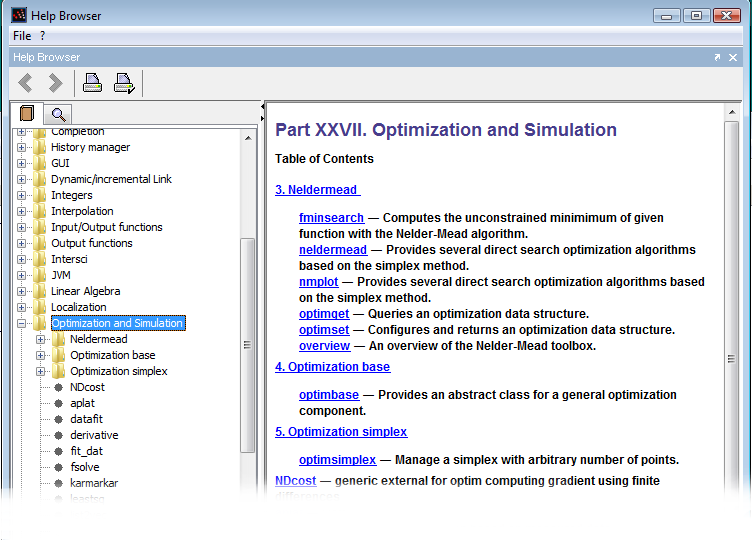
\includegraphics[width=15cm]{introduction/introduction-help.png}
\end{center}
\caption{Built-in help for the Nelder-Mead component}
\label{fig-intro-help}
\end{figure}

\begin{figure}
\begin{center}
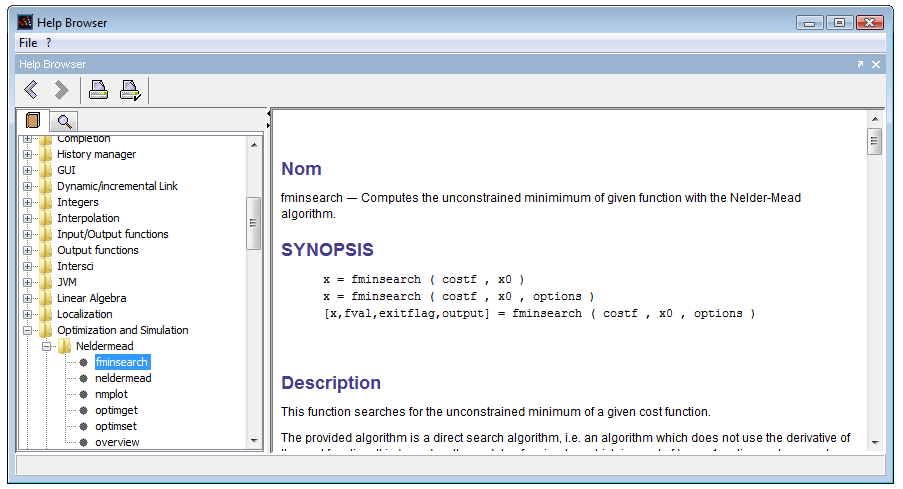
\includegraphics[width=15cm]{introduction/introduction-help-fminsearch.png}
\end{center}
\caption{Built-in help for the \scifunction{fminsearch} function}
\label{fig-intro-helpfminsearch}
\end{figure}

Several demonstrations are provided with the component. These 
are available from the "Demonstration" menu of the Scilab console
and are presented in figure \ref{fig-intro-demos}.

\begin{figure}
\begin{center}
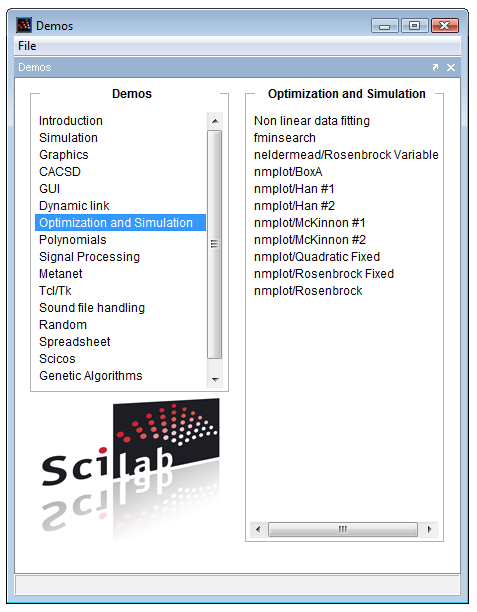
\includegraphics[width=10cm]{introduction/introduction-demos.png}
\end{center}
\caption{Built-in demonstration scripts for the Nelder-Mead component}
\label{fig-intro-demos}
\end{figure}

The following script shows where the demonstration scripts are 
available from the Scilab installation directory.

\lstset{language=scilabscript}
\begin{lstlisting}
-->cd SCI/modules/optimization/demos/neldermead
 ans  =
 
 D:\Programs\SCFD8E~1\modules\optimization\demos\neldermead   
 
-->ls *.sce
 ans  =
 
!nmplot_rosenbrock.sce        !
!                             !
!nmplot_rosenbrock.fixed.sce  !
!                             !
!nmplot_quadratic.fixed.sce   !
!                             !
!nmplot_mckinnon2.sce         !
!                             !
!nmplot_mckinnon.sce          !
!                             !
!nmplot_han2.sce              !
!                             !
!nmplot_han1.sce              !
!                             !
!nmplot_boxproblemA.sce       !
!                             !
!neldermead_rosenbrock.sce    !
!                             !
!neldermead.dem.sce           !
!                             !
!fminsearch.sce               !
\end{lstlisting}

These components were developped based on unit tests, which are 
provided with Scilab.
These unit tests are located in the "SCI/modules/optimization/tests/unit\_tests"
directory, under the "neldermead", "optimsimplex" and "optimbase" directories.
Each unit test correspond to a .tst file. These tests are covering most 
(if not all) the features provided by the components. This is why there are 
a good source of information on how to use the functions.






\section{Quadratic equation}

In this section, we detail the computation of the roots of a quadratic polynomial.
As we shall see, there is a whole world from the mathematics formulas to the 
implementation of such computations. In the first part, we briefly report the formulas which allow to 
compute the real roots of a quadratic equation with real coefficients.
We then present the na�ve algorithm based on these mathematical formulas. 
In the second part, we make some experiments in Scilab and compare our
na�ve algorithm with the \emph{roots} Scilab primitive.
In the third part, we analyse 
why and how floating point numbers must be taken into account when the 
implementation of such roots is required.

\subsection{Theory}

We consider the following quadratic equation, with real 
coefficients $a, b, c \in \RR$ \cite{wikipediaquadratic,wikipedialossofsign,mathworldquadratic} :

\begin{eqnarray}
a x^2 + b x + c = 0.
\end{eqnarray}

The real roots of the quadratic equations are
\begin{eqnarray}
x_- &=& \frac{-b- \sqrt{b^2-4ac}}{2a}, \label{real:x-}\\
x_+ &=& \frac{-b+ \sqrt{b^2-4ac}}{2a}, \label{real:x+}
\end{eqnarray}
with the hypothesis that the discriminant $\Delta=b^2-4ac$
is positive.

The naive, simplified, algorithm which computes the roots of the 
quadratic is presented in figure \ref{naive-quadratic}.

\begin{figure}[htbp]
\begin{algorithmic}
\STATE $\Delta\gets b^2-4ac$
\STATE $s\gets \sqrt{\Delta}$
\STATE $x_-\gets (-b-s)/(2a)$
\STATE $x_+\gets (-b+s)/(2a)$
\end{algorithmic}
\caption{Naive algorithm to compute the real roots of a quadratic equation}
\label{naive-quadratic}
\end{figure}

\subsection{Experiments}

The following Scilab function is a straitforward implementation
of the previous formulas.

\lstset{language=Scilab}
\lstset{numbers=left}
\lstset{basicstyle=\footnotesize}
\lstset{keywordstyle=\bfseries}
\begin{lstlisting}
function r=myroots(p)
  c=coeff(p,0);
  b=coeff(p,1);
  a=coeff(p,2);
  r=zeros(2,1);
  r(1)=(-b+sqrt(b^2-4*a*c))/(2*a);
  r(2)=(-b-sqrt(b^2-4*a*c))/(2*a);
endfunction
\end{lstlisting}

The goal of this section is to show that some additionnal
work is necessary to compute the roots of the quadratic equation
with sufficient accuracy.
We will especially pay attention to rounding errors and 
overflow problems.
In this section, we show that the \emph{roots} command 
of the Scilab language is not \emph{naive}, in the sense that it 
takes into account for the floating point implementation details 
that we will see in the next section.



\subsubsection{Rounding errors}

We analyse the rounding errors which are 
appearing when the discriminant of the quadratic equation 
is such that $b^2\approx 4ac$.
We consider the following quadratic equation 
\begin{eqnarray}
\epsilon x^2 + (1/\epsilon)x - \epsilon = 0
\end{eqnarray}
with $\epsilon=0.0001=10^{-4}$.

The two real solutions of the quadratic equation are
\begin{eqnarray}
x_- &=& \frac{-1/\epsilon- \sqrt{1/\epsilon^2+4\epsilon^2}}{2\epsilon} \approx  -1/\epsilon^2, \\
x_+ &=& \frac{-1/\epsilon+ \sqrt{1/\epsilon^2+4\epsilon^2}}{2\epsilon} \approx  \epsilon^2
\end{eqnarray}

The following Scilab script shows an example of the computation
of the roots of such a polynomial with the \emph{roots}
primitive and with a naive implementation.
Only the positive root $x_+ \approx \epsilon^2$ is considered in this 
test (the $x_-$ root is so that $x_- \rightarrow -\infty$ in both 
implementations).

\lstset{language=Scilab}
\lstset{numbers=left}
\lstset{basicstyle=\footnotesize}
\lstset{keywordstyle=\bfseries}
\begin{lstlisting}
p=poly([-0.0001 10000.0 0.0001],"x","coeff");
e1 = 1e-8;
roots1 = myroots(p);
r1 = roots1(1);
roots2 = roots(p);
r2 = roots2(1);
error1 = abs(r1-e1)/e1;
error2 = abs(r2-e1)/e1;
printf("Expected : %e\n", e1);
printf("Naive method : %e (error=%e)\n", r1,error1);
printf("Scilab method : %e (error=%e)\n", r2, error2);
\end{lstlisting}

The script then prints out :

\begin{verbatim}
Expected : 1.000000e-008
Naive method : 9.094947e-009 (error=9.050530e-002)
Scilab method : 1.000000e-008 (error=1.654361e-016)
\end{verbatim}

The result is surprising, since the naive root has 
no correct digit and a relative error which is 14 orders 
of magnitude greater than the relative error of the Scilab root.

The explanation for such a behaviour is that the expression of the 
positive root is the following 

\begin{eqnarray}
x_+ &=& \frac{-1/\epsilon+ \sqrt{1/\epsilon^2+4\epsilon^2}}{2\epsilon}
\end{eqnarray}

and is numerically evalutated as 

\begin{verbatim}
\sqrt{1/\epsilon^2+4\epsilon^2} = 10000.000000000001818989
\end{verbatim}

As we see, the first digits are correct, but the last digits 
are polluted with rounding errors. When the expression $-1/\epsilon+ \sqrt{1/\epsilon^2+4\epsilon^2}$
is evaluated, the following computations are performed~:

\begin{verbatim}
-1/\epsilon+ \sqrt{1/\epsilon^2+4\epsilon^2} 
  = -10000.0 + 10000.000000000001818989 
  = 0.0000000000018189894035
\end{verbatim}

The user may think that the result is extreme, but it 
is not. Reducing furter the value of $\epsilon$ down to 
$\epsilon=10^{-11}$, we get the following output :

\begin{verbatim}
Expected : 1.000000e-022
Naive method : 0.000000e+000 (error=1.000000e+000)
Scilab method : 1.000000e-022 (error=1.175494e-016)
\end{verbatim}

The relative error is this time 16 orders of magnitude 
greater than the relative error of the Scilab root.
In fact, the naive implementation computes a false root $x_+$ even for 
a value of epsilon equal to $\epsilon=10^-3$, where the relative 
error is 7 times greater than the relative error produced by the 
\emph{roots} primitive.

\subsubsection{Overflow}

In this section, we analyse the overflow exception which is  
appearing when the discriminant of the quadratic equation 
is such that $b^2>> 4ac$.
We consider the following quadratic equation 
\begin{eqnarray}
x^2 + (1/\epsilon)x + 1 = 0
\end{eqnarray}
with $\epsilon\rightarrow 0$.

The roots of this equation are 
\begin{eqnarray}
x_- &\approx& -1/\epsilon \rightarrow -\infty, \qquad \epsilon \rightarrow 0\\
x_+ &\approx& -\epsilon \rightarrow 0^-, \qquad \epsilon \rightarrow 0
\end{eqnarray}
To create a difficult case, we search $\epsilon$ so that 
$1/\epsilon^2 = 10^{310}$, because we know that $10^{308}$
is the maximum value available with double precision floating 
point numbers. One possible solution is $\epsilon=10^{-155}$.

The following Scilab script shows an example of the computation
of the roots of such a polynomial with the \emph{roots}
primitive and with a naive implementation.

\lstset{language=Scilab}
\lstset{numbers=left}
\lstset{basicstyle=\footnotesize}
\lstset{keywordstyle=\bfseries}
\begin{lstlisting}
// Test #3 : overflow because of b
e=1.e-155
a = 1;
b = 1/e;
c = 1;
p=poly([c b a],"x","coeff");
expected = [-e;-1/e];
roots1 = myroots(p);
roots2 = roots(p);
error1 = abs(roots1-expected)/norm(expected);
error2 = abs(roots2-expected)/norm(expected);
printf("Expected : %e %e\n", expected(1),expected(2));
printf("Naive method : %e %e (error=%e)\n", roots1(1),roots1(2),error1);
printf("Scilab method : %e %e (error=%e)\n", roots2(1),roots2(2), error2);
\end{lstlisting}

The script then prints out :

\begin{verbatim}
Expected : -1.000000e-155 -1.000000e+155
Naive method : Inf Inf (error=Nan)
Scilab method : -1.000000e-155 -1.000000e+155 (error=0.000000e+000)
\end{verbatim}

As we see, the $b^2-4ac$ term has been evaluated as $1/\epsilon^2-4$,
which is approximately equal to $10^{310}$. This number cannot 
be represented in a floating point number. It therefore produces the 
IEEE overflow exception and set the result as \emph{Inf}.

\subsection{Explanations}

The following tricks are extracted from the 
\emph{quad} routine of the \emph{RPOLY} algorithm by
Jenkins \cite{Jenkins1975}. This algorithm is used by Scilab in the 
roots primitive, where a special case is handled when the 
degree of the equation is equal to 2, i.e. a quadratic equation.

\subsubsection{Properties of the roots}

One can easily show that the sum and the product of the roots
allow to recover the coefficients of the equation which was solve.
One can show that 
\begin{eqnarray}
x_- + x_+ &=&\frac{-b}{a}\\
x_- x_+ &=&\frac{c}{a}
\end{eqnarray}
Put in another form, one can state that the computed roots are 
solution of the normalized equation 
\begin{eqnarray}
x^2 - \left(\frac{x_- + x_+}{a}\right) x  + x_- x_+ &=&0
\end{eqnarray}

Other transformation leads to an alternative form for the roots. 
The original quadratic equation can be written as a quadratic 
equation on $1/x$
\begin{eqnarray}
c(1/x)^2 + b (1/x)  + a &=&0
\end{eqnarray}
Using the previous expressions for the solution of $ax^2+bx+c=0$ leads to the 
following expression of the roots of the quadratic equation when the 
discriminant is positive 
\begin{eqnarray}
x_- &=& \frac{2c}{-b+ \sqrt{b^2-4ac}}, \label{real:x-inverse}\\
x_+ &=& \frac{2c}{-b- \sqrt{b^2-4ac}} \label{real:x+inverse}
\end{eqnarray}
These roots can also be computed from \ref{real:x-}, with the 
multiplication by $-b+ \sqrt{b^2-4ac}$.

\subsubsection{Conditionning of the problem}

The conditionning of the problem may be evaluated with the 
computation of the partial derivatives of the roots of the 
equations with respect to the coefficients.
These partial derivatives measure the sensitivity of the 
roots of the equation with respect to small errors which might 
pollute the coefficients of the quadratic equations.

In the following, we note $x_-=\frac{-b- \sqrt{\Delta}}{2a}$ 
and $x_+=\frac{-b+ \sqrt{\Delta}}{2a}$ when $a\neq 0$.
If the discriminant is stricly positive and $a\neq 0$, i.e. if the roots 
of the quadratic are real, the partial derivatives of the 
roots are the following :
\begin{eqnarray}
\frac{\partial x_-}{\partial a} &=& \frac{c}{a\sqrt{\Delta}} + \frac{b+\sqrt{\Delta}}{2a^2}, \qquad a\neq 0, \qquad \Delta\neq 0\\
\frac{\partial x_+}{\partial a} &=& -\frac{c}{a\sqrt{\Delta}} + \frac{b-\sqrt{\Delta}}{2a^2}\\
\frac{\partial x_-}{\partial b} &=& \frac{-1-b/\sqrt{\Delta}}{2a}\\
\frac{\partial x_+}{\partial b} &=& \frac{-1+b/\sqrt{\Delta}}{2a}\\
\frac{\partial x_-}{\partial c} &=& \frac{1}{\sqrt{\Delta}}\\
\frac{\partial x_+}{\partial c} &=& -\frac{1}{\sqrt{\Delta}}
\end{eqnarray}

If the discriminant is zero, the partial derivatives of the 
double real root are the following :
\begin{eqnarray}
\frac{\partial x_\pm}{\partial a} &=& \frac{b}{2a^2}, \qquad a\neq 0\\
\frac{\partial x_\pm}{\partial b} &=& \frac{-1}{2a}\\
\frac{\partial x_\pm}{\partial c} &=& 0
\end{eqnarray}

The partial derivates indicate that if $a\approx 0$ or $\Delta\approx 0$,
the problem is ill-conditionned. 



\subsubsection{Floating-Point implementation : fixing rounding error}

In this section, we show how to compute the roots of a 
quadratic equation with protection against rounding 
errors, protection against overflow and a minimum 
amount of multiplications and divisions.

Few but important references deals with floating point
implementations of the roots of a quadratic polynomial.
These references include the important paper \cite{WhatEveryComputerScientist} by Golberg, 
the Numerical Recipes \cite{NumericalRecipes}, chapter 5, section 5.6
and \cite{FORSYTHE1991}, \cite{Nievergelt2003}, \cite{Kahan2004}.

The starting point is the mathematical solution of the quadratic equation, 
depending on the sign of the discriminant $\Delta=b^2 - 4ac$ :
\begin{itemize}
\item If $\Delta> 0$, there are two real roots, 
\begin{eqnarray}
x_\pm &=& \frac{-b\pm \sqrt{\Delta}}{2a}, \qquad a\neq 0
\end{eqnarray}
\item If $\Delta=0$, there are one double root,
\begin{eqnarray}
x_\pm &=& -\frac{b}{2a}, \qquad a\neq 0
\end{eqnarray}
\item If $\Delta< 0$, 
\begin{eqnarray}
x_\pm &=&\frac{-b}{2a} \pm i \frac{\sqrt{-\Delta}}{2a}, \qquad a\neq 0
\end{eqnarray}
\end{itemize}


In the following, we make the hypothesis that $a\neq 0$.

The previous experiments suggest that the floating point implementation
must deal with two different problems :
\begin{itemize}
\item rounding errors when $b^2\approx 4ac$ because of the cancelation of the 
terms which have opposite signs,
\item overflow in the computation of the discriminant $\Delta$ when $b$ is 
large in magnitude with respect to $a$ and $c$.
\end{itemize}

When $\Delta>0$, the rounding error problem can be splitted in two cases
\begin{itemize}
\item if $b<0$, then $-b+\sqrt{b^2-4ac}$ may suffer of rounding errors,
\item if $b>0$, then $-b-\sqrt{b^2-4ac}$ may suffer of rounding errors.
\end{itemize}
 
Obviously, the rounding problem will not appear when $\Delta<0$,
since the complex roots do not use the sum $-b+\sqrt{b^2-4ac}$.
When $\Delta=0$, the double root does not cause further trouble.
The rounding error problem must be solved only when $\Delta>0$ and the 
equation has two real roots.

A possible solution may found in combining the following expressions for the 
roots 
\begin{eqnarray}
x_- &=& \frac{-b- \sqrt{b^2-4ac}}{2a}, \label{real:x-2}\\
x_- &=& \frac{2c}{-b+ \sqrt{b^2-4ac}}, \label{real:x-inverse2}\\
x_+ &=& \frac{-b+ \sqrt{b^2-4ac}}{2a}, \label{real:x+2}\\
x_+ &=& \frac{2c}{-b- \sqrt{b^2-4ac}} \label{real:x+inverse2}
\end{eqnarray}

The trick is to pick the formula so that the sign of $b$ is the 
same as the sign of the square root.

The following choice allow to solve the rounding error problem 
\begin{itemize}
\item compute $x_-$ : if $b<0$, then compute $x_-$ from \ref{real:x-inverse2}, else 
(if $b>0$), compute $x_-$ from \ref{real:x-2},
\item compute $x_+$ : if $b<0$, then compute $x_+$ from \ref{real:x+2}, else 
(if $b>0$), compute $x_+$ from \ref{real:x+inverse2}.
\end{itemize}

The solution of the rounding error problem  can be adressed, by considering the 
modified Fagnano formulas
\begin{eqnarray}
x_1 &=& -\frac{2c}{b+sgn(b)\sqrt{b^2-4ac}}, \\
x_2 &=& -\frac{b+sgn(b)\sqrt{b^2-4ac}}{2a}, 
\end{eqnarray}
where 
\begin{eqnarray}
sgn(b)=\left\{\begin{array}{l}
1, \textrm{ if } b\geq 0,\\
-1, \textrm{ if } b< 0,
\end{array}\right.
\end{eqnarray}
The roots $x_{1,2}$ correspond to $x_{+,-}$ so that if $b<0$, $x_1=x_-$ and
if $b>0$, $x_1=x_+$. On the other hand, if $b<0$, $x_2=x_+$ and
if $b>0$, $x_2=x_-$.

An additionnal remark is that the division by two (and the multiplication
by 2) is exact with floating point numbers so these operations
cannot be a source of problem. But it is 
interesting to use $b/2$, which involves only one division, instead
of the three multiplications $2*c$, $2*a$ and $4*a*c$.
This leads to the following expressions of the real roots 
\begin{eqnarray}
x_- &=& -\frac{c}{(b/2)+sgn(b)\sqrt{(b/2)^2-ac}}, \\
x_+ &=& -\frac{(b/2)+sgn(b)\sqrt{(b/2)^2-ac}}{a}, 
\end{eqnarray}
which can be simplified into
\begin{eqnarray}
b'&=&b/2\\
h&=& -\left(b'+sgn(b)\sqrt{b'^2-ac}\right)\\
x_1 &=& \frac{c}{h}, \\
x_2 &=& \frac{h}{a}, 
\end{eqnarray}
where the discriminant is positive, i.e. $b'^2-ac>0$.

One can use the same value $b'=b/2$ with the complex roots in the 
case where the discriminant is negative, i.e. $b'^2-ac<0$ :
\begin{eqnarray}
x_1 &=& -\frac{b'}{a} - i \frac{\sqrt{ac-b'^2}}{a}, \\
x_2 &=& -\frac{b'}{a} + i \frac{\sqrt{ac-b'^2}}{a}, 
\end{eqnarray}

A more robust algorithm, based on the previous analysis is presented in figure \ref{robust-quadratic}.
By comparing \ref{naive-quadratic} and \ref{robust-quadratic}, we can see that 
the algorithms are different in many points.

\begin{figure}[htbp]
\begin{algorithmic}
\IF {$a=0$}
        \IF {$b=0$}
            \STATE $x_-\gets 0$
            \STATE $x_+\gets 0$
        \ELSE
            \STATE $x_-\gets -c/b$
            \STATE $x_+\gets 0$
        \ENDIF
\ELSIF {$c=0$}
        \STATE $x_-\gets -b/a$
        \STATE $x_+\gets 0$        
\ELSE
        \STATE $b'\gets b/2$
        \STATE $\Delta\gets b'^2 - ac$
        \IF {$\Delta<0$}
                \STATE $s\gets \sqrt{-\Delta}$
                \STATE $x_1^R\gets -b'/a$
                \STATE $x_1^I\gets -s/a$
                \STATE $x_2^R\gets x_-^R$
                \STATE $x_2^I\gets -x_1^I$
        \ELSIF {$\Delta=0$}
                \STATE $x_1\gets -b'/a$
                \STATE $x_2\gets x_2$
        \ELSE
                \STATE $s\gets \sqrt{\Delta}$
                \IF {$b>0$}
                    \STATE $g=1$
                \ELSE
                    \STATE $g=-1$
                \ENDIF
                \STATE $h=-(b'+g*s)$
                \STATE $x_1\gets c/h$
                \STATE $x_2\gets h/a$
        \ENDIF
\ENDIF 
\end{algorithmic}
\caption{A more robust algorithm to compute the roots of a quadratic equation}
\label{robust-quadratic}
\end{figure}

\subsubsection{Floating-Point implementation : fixing overflow problems}

The remaining problem is to compute $b'^2-ac$ without creating 
unnecessary overflows. 

Notice that a small improvment
has allread been done : if $|b|$ is close to the upper bound $10^{154}$, 
then $|b'|$ may be less difficult to process since $|b'|=|b|/2 < |b|$.
One can then compute the square root by using normalization methods, 
so that the overflow problem can be drastically reduced.
The method is based on the fact that the term $b'^2-ac$ can be 
evaluted with two equivalent formulas
\begin{eqnarray}
b'^2-ac &=& b'^2\left[1-(a/b')(c/b')\right] \\
b'^2-ac &=& c\left[b'(b'/c) - a\right]
\end{eqnarray}

\begin{itemize}
\item If $|b'|>|c|>0$, then the expression involving $\left(1-(a/b')(c/b')\right)$
is so that no overflow is possible since $|c/b'| < 1$ and the problem occurs
only when $b$ is large in magnitude with respect to $a$ and $c$.
\item If $|c|>|b'|>0$, then the expression involving $\left(b'(b'/c) - a\right)$
should limit the possible overflows since $|b'/c| < 1$.
\end{itemize}
These normalization tricks are similar to the one used by Smith in the 
algorithm for the division of complex numbers \cite{Smith1962}.

\subsection{References}

The 1966 technical report by G. Forsythe \cite{Forsythe1966} 
presents the floating point system and the possible large error 
in using mathematical algorithms blindly. An accurate way of solving 
a quadratic is outlined. A few general remarks are made about 
computational mathematics. The 1991 paper by Goldberg 
\cite{WhatEveryComputerScientist} is a general presentation of the floating
point system and its consequences. It begins with background on floating point 
representation and rounding errors, continues with a discussion
of the IEEE floating point standard and concludes with examples of how
computer system builders can better support floating point. The section
1.4, "Cancellation" specificaly consider the computation of the roots
of a quadratic equation.
One can also consult the experiments performed by Nievergelt in \cite{Nievergelt2003}.




\section{Numerical derivatives}

In this section, we detail the computation of the numerical derivative of 
a given function.

In the first part, we briefly report the first order forward formula, which 
is based on the Taylor theorem.
We then present the na�ve algorithm based on these mathematical formulas. 
In the second part, we make some experiments in Scilab and compare our
na�ve algorithm with the \emph{derivative} Scilab primitive.
In the third part, we analyse 
why and how floating point numbers must be taken into account when the 
numerical derivatives are to compute.

\subsection{Theory}

The basic result is the Taylor formula with one variable \cite{dixmier}

\begin{eqnarray}
f(x+h) &=& f(x) 
+ h f^\prime(x)
+\frac{h^2}{2} f^{\prime \prime}(x)
+\frac{h^3}{6} f^{\prime \prime \prime}(x)
+\frac{h^4}{24} f^{\prime \prime \prime \prime}(x) + \mathcal{O}(h^5)
\end{eqnarray}

If we write the Taylor formulae of a one variable function $f(x)$ 
\begin{eqnarray}
f(x+h) &\approx& f(x) + h \frac{\partial f}{\partial x}+ \frac{h^2}{2} f^{\prime \prime}(x)
\end{eqnarray}
we get the forward difference which approximates the first derivate at order 1 
\begin{eqnarray}
f^\prime(x) &\approx& \frac{f(x+h)  - f(x)}{h} + \frac{h}{2} f^{\prime \prime}(x)
\end{eqnarray}

The naive algorithm to compute the numerical derivate of 
a function of one variable is presented in figure \ref{naive-numericalderivative}.

\begin{figure}[htbp]
\begin{algorithmic}
\STATE $f'(x) \gets (f(x+h)-f(x))/h$
\end{algorithmic}
\caption{Naive algorithm to compute the numerical derivative of a function of one variable}
\label{naive-numericalderivative}
\end{figure}

\subsection{Experiments}

The following Scilab function is a straitforward implementation
of the previous algorithm.

\lstset{language=Scilab}
\lstset{numbers=left}
\lstset{basicstyle=\footnotesize}
\lstset{keywordstyle=\bfseries}
\begin{lstlisting}
function fp = myfprime(f,x,h)
  fp = (f(x+h) - f(x))/h;
endfunction
\end{lstlisting}

In our experiments, we will compute the derivatives of the 
square function $f(x)=x^2$, which is $f'(x)=2x$.
The following Scilab script implements the square function.

\lstset{language=Scilab}
\lstset{numbers=left}
\lstset{basicstyle=\footnotesize}
\lstset{keywordstyle=\bfseries}
\begin{lstlisting}
function y = myfunction (x)
  y = x*x;
endfunction
\end{lstlisting}

The most na�ve idea is that the computed relative error 
is small when the step $h$ is small. Because \emph{small}
is not a priori clear, we take $\epsilon\approx 10^{-16}$
in double precision as a good candidate for \emph{small}.
In the following script, we compare the computed 
relative error produced by our na�ve method with step
$h=\epsilon$ and the \emph{derivative} primitive with
default step.

\lstset{language=Scilab}
\lstset{numbers=left}
\lstset{basicstyle=\footnotesize}
\lstset{keywordstyle=\bfseries}
\begin{lstlisting}
x = 1.0;
fpref = derivative(myfunction,x,order=1);
e = abs(fpref-2.0)/2.0;
mprintf("Scilab f''=%e, error=%e\n", fpref,e);
h = 1.e-16;
fp = myfprime(myfunction,x,h);
e = abs(fp-2.0)/2.0;
mprintf("Naive f''=%e, h=%e, error=%e\n", fp,h,e);
\end{lstlisting}

When executed, the previous script prints out :

\begin{verbatim}
Scilab f'=2.000000e+000, error=7.450581e-009
Naive f'=0.000000e+000, h=1.000000e-016, error=1.000000e+000
\end{verbatim}

Our na�ve method seems to be quite inaccurate and has not 
even 1 significant digit !
The Scilab primitive, instead, has 9 significant digits.

Since our faith is based on the truth of the mathematical
theory, some deeper experiments must be performed.
We then make the following experiment, by taking an
initial step $h=1.0$ and then dividing $h$ by 10 at each
step of a loop with 20 iterations.

\lstset{language=Scilab}
\lstset{numbers=left}
\lstset{basicstyle=\footnotesize}
\lstset{keywordstyle=\bfseries}
\begin{lstlisting}
x = 1.0;
fpref = derivative(myfunction,x,order=1);
e = abs(fpref-2.0)/2.0;
mprintf("Scilab f''=%e, error=%e\n", fpref,e);
h = 1.0;
for i=1:20
  h=h/10.0;
  fp = myfprime(myfunction,x,h);
  e = abs(fp-2.0)/2.0;
  mprintf("Naive f''=%e, h=%e, error=%e\n", fp,h,e);
end
\end{lstlisting}

Scilab then produces the following output.

\begin{verbatim}
Scilab f'=2.000000e+000, error=7.450581e-009
Naive f'=2.100000e+000, h=1.000000e-001, error=5.000000e-002
Naive f'=2.010000e+000, h=1.000000e-002, error=5.000000e-003
Naive f'=2.001000e+000, h=1.000000e-003, error=5.000000e-004
Naive f'=2.000100e+000, h=1.000000e-004, error=5.000000e-005
Naive f'=2.000010e+000, h=1.000000e-005, error=5.000007e-006
Naive f'=2.000001e+000, h=1.000000e-006, error=4.999622e-007
Naive f'=2.000000e+000, h=1.000000e-007, error=5.054390e-008
Naive f'=2.000000e+000, h=1.000000e-008, error=6.077471e-009
Naive f'=2.000000e+000, h=1.000000e-009, error=8.274037e-008
Naive f'=2.000000e+000, h=1.000000e-010, error=8.274037e-008
Naive f'=2.000000e+000, h=1.000000e-011, error=8.274037e-008
Naive f'=2.000178e+000, h=1.000000e-012, error=8.890058e-005
Naive f'=1.998401e+000, h=1.000000e-013, error=7.992778e-004
Naive f'=1.998401e+000, h=1.000000e-014, error=7.992778e-004
Naive f'=2.220446e+000, h=1.000000e-015, error=1.102230e-001
Naive f'=0.000000e+000, h=1.000000e-016, error=1.000000e+000
Naive f'=0.000000e+000, h=1.000000e-017, error=1.000000e+000
Naive f'=0.000000e+000, h=1.000000e-018, error=1.000000e+000
Naive f'=0.000000e+000, h=1.000000e-019, error=1.000000e+000
Naive f'=0.000000e+000, h=1.000000e-020, error=1.000000e+000
\end{verbatim}

We see that the relative error begins by decreasing, and then 
is increasing.
Obviously, the optimum step is approximately $h=10^{-8}$, where the
relative error is approximately $e_r=6.10^{-9}$. 
We should not be surprised to see that Scilab has computed 
a derivative which is near the optimum.

\subsection{Explanations}

\subsubsection{Floating point implementation}

With a floating point computer, the total 
error that we get from the forward difference approximation
is (skipping the multiplication constants) the sum of the 
linearization error $E_l = h$ (i.e. the $\mathcal{O}(h)$ term)
and the rounding error $rf(x)$ on the difference $f(x+h)  - f(x)$
\begin{eqnarray}
E = \frac{rf(x)}{h} + \frac{h}{2} f^{\prime \prime}(x)
\end{eqnarray}
When $h\rightarrow \infty$, the error is then the sum of a
term which converges toward $+\infty$ and a term which converges toward 0.
The total error is minimized when both terms are equal.
With a single precision computation, the rounding error is $r = 10^{-7}$
and with a double precision computation, the rounding error is $r = 10^{-16}$.
We make here the assumption that the values $f(x)$ and 
$f^{\prime \prime}(x)$ are near 1 so that the error can be written 
\begin{eqnarray}
E = \frac{r}{h} + h
\end{eqnarray}
We want to compute the step $h$ from the rounding error $r$ with a 
step satisfying 
\begin{eqnarray}
h = r^\alpha
\end{eqnarray}
for some $\alpha > 0$.
The total error is therefore 
\begin{eqnarray}
E = r^{1-\alpha} + r^\alpha
\end{eqnarray}
The total error is minimized when both terms are equal, that is, 
when the exponents are equal  $1-\alpha = \alpha$ which leads to 
\begin{eqnarray}
\alpha = \frac{1}{2}
\end{eqnarray}
We conclude that the step which minimizes the error is 
\begin{eqnarray}
h = r^{1/2}
\end{eqnarray}
and the associated error is 
\begin{eqnarray}
E = 2 r^{1/2}
\end{eqnarray}

Typical values with single precision are $h = 10^{-4}$ and $E=2. 10^{-4}$
and with double precision $h = 10^{-8}$ and $E=2. 10^{-8}$.
These are the minimum error which are achievable with a forward difference
numerical derivate.

To get a significant value of the step $h$, the step is computed
with respect to the point where the derivate is to compute
\begin{eqnarray}
h = r^{1/2} x
\end{eqnarray}

One can generalize the previous computation with the 
assumption that the scaling parameter from the Taylor 
expansion is $h^{\alpha_1}$ and the order of the formula
is $\mathcal{O}(h^{\alpha_2})$. The total error is then 
\begin{eqnarray}
E = \frac{r}{h^{\alpha_1}} + h^{\alpha_2}
\end{eqnarray}
The optimal step is then 
\begin{eqnarray}
h = r^{\frac{1}{\alpha_1 + \alpha_2}}
\end{eqnarray}
and the associated error is 
\begin{eqnarray}
E = 2 r^{\frac{\alpha_2}{\alpha_1 + \alpha_2}}
\end{eqnarray}


An additional trick \cite{NumericalRecipes} is to compute the 
step $h$ so that the rounding error for the sum $x+h$ is minimum.
This is performed by the following algorithm, which implies a temporary 
variable $t$
\begin{eqnarray}
t = x + h\\
h = t - h
\end{eqnarray}


\subsubsection{Results}

In the following results, the variable $x$ is either a 
scalar $x^in \RR$ or a vector $x\in \RR^n$.
When $x$ is a vector, the step $h_i$ is defined by
\begin{eqnarray}
h_i = (0,\ldots,0,1,0,\ldots,0)
\end{eqnarray}
so that the only non-zero component of $h_i$ is the $i$-th component.

\begin{itemize}

\item First derivate : forward 2 points 
\begin{eqnarray}
f^\prime(x) &\approx& \frac{f(x+h)  - f(x)}{h} + \mathcal{O}(h)
\end{eqnarray}
Optimal step : $h = r^{1/2}$ and error $E=2r^{1/2}$.\\
Single precision : $h \approx 10^{-4}$ and $E\approx 10^{-4}$.\\
Double precision $h \approx 10^{-8}$ and $E\approx 10^{-8}$.

\item First derivate : backward 2 points 
\begin{eqnarray}
f^\prime(x) &\approx& \frac{f(x) - f(x-h)}{h} + \mathcal{O}(h)
\end{eqnarray}
Optimal step : $h = r^{1/2}$ and error $E=2r^{1/2}$.\\
Single precision : $h \approx 10^{-4}$ and $E\approx 10^{-4}$.\\
Double precision $h \approx 10^{-8}$ and $E\approx 10^{-8}$.

\item First derivate : centered 2 points 
\begin{eqnarray}
f^\prime(x) &\approx& \frac{f(x+h) - f(x-h)}{2h} + \mathcal{O}(h^2)
\end{eqnarray}
Optimal step : $h = r^{1/3}$ and error $E=2r^{2/3}$.\\
Single precision : $h \approx 10^{-3}$ and $E\approx 10^{-5}$.\\
Double precision $h \approx 10^{-5}$ and $E\approx 10^{-10}$.

\end{itemize}

\subsubsection{Robust algorithm}

The robust algorithm to compute the numerical derivate of 
a function of one variable is presented in figure \ref{robust-numericalderivative}.

\begin{figure}[htbp]
\begin{algorithmic}
\STATE $h \gets \sqrt{\epsilon}$
\STATE $f'(x) \gets (f(x+h)-f(x))/h$
\end{algorithmic}
\caption{A more robust algorithm to compute the numerical derivative of a function of one variable}
\label{robust-numericalderivative}
\end{figure}

\subsection{One more step}

In this section, we analyse the behaviour of \emph{derivative}
when the point $x$ is either large $x \rightarrow \infty$, 
when $x$ is small $x \rightarrow 0$ and when $x = 0$.
We compare these results with the \emph{numdiff} command,
which does not use the same step strategy. As we are going 
to see, both commands performs the same when $x$ is near 1, but 
performs very differently when x is large or small.

We have allready explained the theory of the floating 
point implementation of the \emph{derivative} command.
Is it completely \emph{bulletproof} ? Not exactly. 

See for example the following Scilab session, where one computes the 
numerical derivative of $f(x)=x^2$ for $x=10^{-100}$. The 
expected result is $f'(x) = 2. \times 10^{-100}$.

\begin{verbatim}
-->fp = derivative(myfunction,1.e-100,order=1)
 fp  =
    0.0000000149011611938477  
-->fe=2.e-100
 fe  =
    2.000000000000000040-100  
-->e = abs(fp-fe)/fe
 e  =
    7.450580596923828243D+91  
\end{verbatim}

The result does not have any significant digits.

The explanation is that the step is computed with $h = \sqrt{eps}\approx 10^{-8}$.
Then $f(x+h)=f(10^{-100} + 10^{-8}) \approx f(10^{-8}) = 10^{-16}$, because the 
term $10^{-100}$ is much smaller than $10^{-8}$. The result of the 
computation is therefore $(f(x+h) - f(x))/h = (10^{-16} + 10^{-200})/10^{-8} \approx 10^{-8}$.

The additionnal experiment 

\begin{verbatim}
-->sqrt(%eps)
 ans  =
    0.0000000149011611938477  
\end{verbatim}

allows to check that the result of the computation simply is $\sqrt{eps}$.
That experiment shows that the \emph{derivative} command uses a 
wrong defaut step $h$ when $x$ is very small.

To improve the accuracy of the computation, one can take control of the 
step $h$. A reasonable solution is to use $h=\sqrt{\epsilon}|x|$ so that the 
step is scaled depending on $x$. 
The following script illustrates than method, which produces 
results with 8 significant digits.

\begin{verbatim}
-->fp = derivative(myfunction,1.e-100,order=1,h=sqrt(%eps)*1.e-100)
 fp  =
    2.000000013099139394-100  
-->fe=2.e-100
 fe  =
    2.000000000000000040-100  
-->e = abs(fp-fe)/fe
 e  =
    0.0000000065495696770794  
\end{verbatim}

But when $x$ is exactly zero, the scaling method cannot work, because 
it would produce the step $h=0$, and therefore a division by zero
exception. In that case, the default step provides a good accuracy.

Another command is available in Scilab to compute the 
numerical derivatives of a given function, that is \emph{numdiff}.
The \emph{numdiff} command uses the step 
\begin{eqnarray}
h=\sqrt{\epsilon}(1+10^{-3}|x|).
\end{eqnarray}
In the following paragraphs, we try to analyse why this formula 
has been chosen. As we are going to check experimentally, this step
formula performs better than \emph{derivative} when $x$ is 
large.

As we can see the following session, the behaviour is approximately 
the same when the value of $x$ is 1.

\begin{verbatim}
-->fp = numdiff(myfunction,1.0)
 fp  =
    2.0000000189353417390237  
-->fe=2.0
 fe  =
    2.  
-->e = abs(fp-fe)/fe
 e  =
    9.468D-09  
\end{verbatim}

The accuracy is slightly decreased with respect to the optimal
value 7.450581e-009 which was produced by derivative. But the number 
of significant digits is approximately the same, i.e. 9 digits.

The goal of this step is to produce good accuracy when the value of $x$ 
is large, where the \emph{numdiff} command produces accurate
results, while \emph{derivative} performs poorly.

\begin{verbatim}
-->numdiff(myfunction,1.e10)
  ans  =
    2.000D+10  
-->derivative(myfunction,1.e10,order=1)
 ans  =
    0.  
\end{verbatim}

This step is a trade-off because it allows to keep a good accuracy with
large values of $x$, but produces a slightly sub-optimal step size when 
$x$ is near 1. The behaviour near zero is the same, i.e. both commands 
produce wrong results when $x \rightarrow 0$ and $x\neq 0$.

\subsection{References}

A reference for numerical derivates 
is \cite{AbramowitzStegun1972}, chapter 25. "Numerical Interpolation, 
Differentiation and Integration" (p. 875).
The webpage \cite{schimdtnd} and the book \cite{NumericalRecipes} give
results about the rounding errors.




\section{Complex division}

In that section, we analyse the problem of the complex division in Scilab.
We especially detail the difference between the mathematical, straitforward
formula and the floating point implementation. In the first part, we briefly report 
the formulas which allow to 
compute the real and imaginary parts of the division of two complex numbers.
We then present the na�ve algorithm based on these mathematical formulas. 
In the second part, we make some experiments in Scilab and compare our
na�ve algorithm with the \emph{/} Scilab operator.
In the third part, we analyse 
why and how floating point numbers must be taken into account when the 
implementation of such division is required.

\subsection{Theory}

The formula which allows to compute the 
real and imaginary parts of the division of two 
complex numbers is 
\begin{eqnarray}
\frac{a + ib}{c + id} = \frac{ac + bd}{c^2 + d^2} + i \frac{bc - ad}{c^2 + d^2} 
\end{eqnarray}

The naive algorithm for the computation of the complex division
is presented in figure \ref{naive-complexdivision}.

\begin{figure}[htbp]
\begin{algorithmic}
\STATE $den \gets c^2 + d^2$
\STATE $e \gets (ac + bd)/ den$
\STATE $f \gets (bc - ad)/ den$ 
\end{algorithmic}
\caption{Naive algorithm to compute the complex division}
\label{naive-complexdivision}
\end{figure}


\subsection{Experiments}

The following Scilab function is a straitforward implementation
of the previous formulas.

\lstset{language=Scilab}
\lstset{numbers=left}
\lstset{basicstyle=\footnotesize}
\lstset{keywordstyle=\bfseries}
\begin{lstlisting}
// 
// naive --
//   Compute the complex division with a naive method.
//
function [cr,ci] = naive (ar , ai , br , bi )
  den = br * br + bi * bi;
  cr = (ar * br + ai * bi) / den;
  ci = (ai * br - ar * bi) / den;
endfunction
\end{lstlisting}

In the following script, one compares the naive implementation
against the Scilab implementation with two cases.

\lstset{language=Scilab}
\lstset{numbers=left}
\lstset{basicstyle=\footnotesize}
\lstset{keywordstyle=\bfseries}
\begin{lstlisting}
  // Check that no obvious bug is in mathematical formula.
  [cr ci] = naive ( 1.0 , 2.0 , 3.0 , 4.0 )
  (1.0 + 2.0 * %i)/(3.0 + 4.0 * %i)
  // Check that mathematical formula does not perform well
  // when large number are used.
  [cr ci] = naive ( 1.0 , 1.0 , 1.0 , 1.e307 )
  (1.0 + 1.0 * %i)/(1.0 + 1.e307 * %i)
\end{lstlisting}

That prints out the following messages.

\begin{verbatim}
-->  // Check that no obvious bug is in mathematical formula.
-->  [cr ci] = naive ( 1.0 , 2.0 , 3.0 , 4.0 )
 ci  =
    0.08  
 cr  =
    0.44  
-->  (1.0 + 2.0 * %i)/(3.0 + 4.0 * %i)
 ans  =
    0.44 + 0.08i  
-->  // Check that mathematical formula does not perform well
-->  // when large number are used.
-->  [cr ci] = naive ( 1.0 , 1.0 , 1.0 , 1.e307 )
 ci  =
    0.  
 cr  =
    0.  
-->  (1.0 + 1.0 * %i)/(1.0 + 1.e307 * %i)
 ans  =
    1.000-307 - 1.000-307i  
\end{verbatim}

The simple calculation confirms that there is no bug in the 
naive implementation. But differences are apprearing when 
large numbers are used. In the second case, the naive 
implementation does not give a single exact digit !

To make more complete tests, the following script allows to 
compare the results of the naive and the Scilab methods.
We use three kinds of relative errors 
\begin{enumerate}
\item the relative error on the complex numbers, as a whole $e=\frac{|e - c|}{|e|}$,
\item the relative error on the real part $e=\frac{|e_r - e_r|}{e_r}$,
\item the relative error on the imaginary part $e=\frac{|e_i - e_i|}{e_i}$.
\end{enumerate}

\lstset{language=Scilab}
\lstset{numbers=left}
\lstset{basicstyle=\footnotesize}
\lstset{keywordstyle=\bfseries}
\begin{lstlisting}
// 
// compare --
//   Compare 3 methods for complex division:
//   * naive method
//   * Smith method
//   * C99 method
//
function compare (ar, ai, br, bi, rr, ri)
  printf("****************\n");
  printf("           a = %10.5e +  %10.5e * I\n" , ar ,  ai );
  printf("           b = %10.5e +  %10.5e * I\n" , br ,  bi );
  [cr ci] = naive ( ar, ai, br, bi);
  printf("Naive  --> c = %10.5e +  %10.5e * I\n" , cr ,  ci );
  c = cr + %i * ci
  r = rr + %i * ri;
  error1 = abs(r - c)/abs(r);
  if (rr==0.0) then
    error2 = abs(rr - cr);
  else
    error2 = abs(rr - cr)/abs(rr);
  end
  if (ri==0.0) then
    error3 = abs(ri - ci);
  else
    error3 = abs(ri - ci)/abs(ri);
  end
  printf("   e1 = %10.5e, e2 = %10.5e, e3 = %10.5e\n", error1, error2, error3);
  
  a = ar + ai * %i;
  b = br + bi * %i;
  c = a/b;
  cr = real(c);
  ci = imag(c);
  printf("Scilab --> c = %10.5e +  %10.5e * I\n" , cr ,  ci );
  c = cr + %i * ci
  error1 = abs(r - c)/abs(r);
  if (rr==0.0) then
    error2 = abs(rr - cr);
  else
    error2 = abs(rr - cr)/abs(rr);
  end
  if (ri==0.0) then
    error3 = abs(ri - ci);
  else
    error3 = abs(ri - ci)/abs(ri);
  end
  printf("   e1 = %10.5e, e2 = %10.5e, e3 = %10.5e\n", error1, error2, error3);
endfunction
\end{lstlisting}

In the following script, we compare the naive and the Scilab
implementations of the complex division with 4 couples of 
complex numbers. The first instruction "ieee(2)" configures the 
IEEE system so that Inf and Nan numbers are generated instead 
of Scilab error messages.

\lstset{language=Scilab}
\lstset{numbers=left}
\lstset{basicstyle=\footnotesize}
\lstset{keywordstyle=\bfseries}
\begin{lstlisting}
ieee(2);
// Check that naive implementation does not have a bug
ar = 1;
ai = 2;
br = 3;
bi = 4;
rr = 11/25;
ri = 2/25;
compare (ar, ai, br, bi, rr, ri);

// Check that naive implementation is not robust with respect to overflow
ar = 1;
ai = 1;
br = 1;
bi = 1e307;
rr = 1e-307;
ri = -1e-307;
compare (ar, ai, br, bi, rr, ri);

// Check that naive implementation is not robust with respect to underflow
ar = 1;
ai = 1;
br = 1e-308;
bi = 1e-308;
rr = 1e308;
ri = 0.0;
compare (ar, ai, br, bi, rr, ri);

\end{lstlisting}

The script then prints out the following messages.

\begin{verbatim}
****************
           a = 1.00000e+000 +  2.00000e+000 * I
           b = 3.00000e+000 +  4.00000e+000 * I
Naive  --> c = 4.40000e-001 +  8.00000e-002 * I
   e1 = 0.00000e+000, e2 = 0.00000e+000, e3 = 0.00000e+000
Scilab --> c = 4.40000e-001 +  8.00000e-002 * I
   e1 = 0.00000e+000, e2 = 0.00000e+000, e3 = 0.00000e+000
****************
           a = 1.00000e+000 +  1.00000e+000 * I
           b = 1.00000e+000 +  1.00000e+307 * I
Naive  --> c = 0.00000e+000 +  -0.00000e+000 * I
   e1 = 1.00000e+000, e2 = 1.00000e+000, e3 = 1.00000e+000
Scilab --> c = 1.00000e-307 +  -1.00000e-307 * I
   e1 = 2.09614e-016, e2 = 1.97626e-016, e3 = 1.97626e-016
****************
           a = 1.00000e+000 +  1.00000e+000 * I
           b = 1.00000e-308 +  1.00000e-308 * I
Naive  --> c = Inf +  Nan * I
   e1 = Nan, e2 = Inf, e3 = Nan
Scilab --> c = 1.00000e+308 +  0.00000e+000 * I
   e1 = 0.00000e+000, e2 = 0.00000e+000, e3 = 0.00000e+000
\end{verbatim}

The case \#2 and \#3 shows very surprising results.
With case \#2, the relative errors shows that the naive 
implementation does not give any correct digits.
In case \#3, the naive implementation produces Nan and Inf results.
In both cases, the Scilab command "/" gives accurate results, i.e.,
with at least 16 significant digits.

\subsection{Explanations}

In this section, we analyse the reason why the naive implementation
of the complex division leads to unaccurate results.
In the first section, we perform algebraic computations 
and shows the problems of the naive formulas.
In the second section, we present the Smith's method.

\subsubsection{Algebraic computations}

Let's analyse the second test and check the division of test \#2 :

\begin{eqnarray}
\frac{1 + I}{1 + 10^{307} I } = 10^{307} - I * 10^{-307}
\end{eqnarray}

The naive formulas leads to the following results.

\begin{eqnarray}
den &=& c^2 + d^2 = 1^2 + (10^{307})^2 = 1 + 10^{614} \approx 10^{614} \\
e &=& (ac + bd)/ den = (1*1 + 1*10^{307})/1e614 \approx 10^{307}/10^{614} \approx 10^{-307}\\
f &=& (bc - ad)/ den = (1*1 - 1*10^{307})/1e614 \approx -10^{307}/10^{614} \approx -10^{-307}
\end{eqnarray}

To understand what happens with the naive implementation, one should
focus on the intermediate numbers.
If one uses the naive formula with double precision numbers, then

\begin{eqnarray}
den = c^2 + d^2 = 1^2 + (10^{307})^2 = Inf
\end{eqnarray}

This generates an overflow, because $(10^{307})^2 = 10^{614}$ is not representable
as a double precision number.

The $e$ and $f$ terms are then computed as 

\begin{eqnarray}
e = (ac + bd)/ den = (1*1 + 1*10^{307})/Inf = 10^{307}/Inf = 0\\
f = (bc - ad)/ den = (1*1 - 1*10^{307})/Inf = -10^{307}/Inf = 0
\end{eqnarray}

The result is then computed without any single correct digit,
even though the initial numbers are all representable as double precision
numbers.

Let us check that the case \#3 is associated with an underflow.
We want to compute the following complex division :

\begin{eqnarray}
\frac{1 + I}{10^{-308} +  10^{-308} I}= 10^{308}
\end{eqnarray}

The naive mathematical formula gives 

\begin{eqnarray}
den &=& c^2 + d^2 = (10^{-308})^2 + (10^{-308})^2 = 10^{-616}10^{-616} + 10^{-616} = 2 \times 10^{-616} \\
e &=& (ac + bd)/ den = (1*10^{-308} + 1*10^{-308})/(2 \times 10^{-616}) \\
 &\approx&  (2 \times 10^{-308})/(2 \times 10^{-616}) \approx 10^{-308} \\
f &=& (bc - ad)/ den = (1*10^{-308} - 1*10^{-308})/(2 \times 10^{-616}) \approx 0/10^{-616} \approx 0
\end{eqnarray}

With double precision numbers, the computation is not performed this way.
Terms which are lower than $10^{-308}$ are too small to be representable 
in double precision and will be reduced to 0 so that an underflow occurs.

\begin{eqnarray}
den &=& c^2 + d^2 = (10^{-308})^2 + (10^{-308})^2 = 10^{-616} + 10^{-616} = 0 \\
e &=& (ac + bd)/ den = (1*10^{-308} + 1*10^{-308})/0 \approx 2\times 10^{-308}/0 \approx Inf \\
f &=& (bc - ad)/ den = (1*10^{-308} - 1*10^{-308})/0 \approx 0/0 \approx NaN \\
\end{eqnarray}

\subsubsection{The Smith's method}

In this section, we analyse the Smith's method and present the detailed
steps of this algorithm in the cases \#2 and \#3.

In Scilab, the algorithm which allows to perform the complex 
division is done by the the \emph{wwdiv} routine, which implements the 
Smith's method \cite{368661}, \cite{WhatEveryComputerScientist}.
The Smith's algorithm is based on normalization, which allow to 
perform the division even if the terms are large. 

The starting point of the method is the mathematical definition 

\begin{eqnarray}
\frac{a + ib}{c + id} = \frac{ac + bd}{c^2 + d^2} + i \frac{bc - ad}{c^2 + d^2} 
\end{eqnarray}

The method of Smith is based on the rewriting of this formula in 
two different, but mathematically equivalent formulas. The basic 
trick is to make the terms $d/c$ or $c/d$ appear in the formulas.
When $c$ is larger than $d$, the formula involving $d/c$ is used.
Instead, when $d$ is larger than $c$, the formula involving $c/d$ is 
used. That way, the intermediate terms in the computations rarely 
exceeds the overflow limits.

Indeed, the complex division formula can be written as 
\begin{eqnarray}
\frac{a + ib}{c + id} = \frac{a + b(d/c)}{c + d(d/c)} + i \frac{b - a(d/c)}{c + d(d/c)} \\
\frac{a + ib}{c + id} = \frac{a(c/d) + b}{c(d/c) + d} + i \frac{b(c/d) - a}{c(d/c) + d} 
\end{eqnarray}

These formulas can be simplified as 

\begin{eqnarray}
\frac{a + ib}{c + id} = \frac{a + br}{c + dr} + i \frac{b - ar}{c + dr}, \qquad r = d/c \\
\frac{a + ib}{c + id} = \frac{ar + b}{cr + d} + i \frac{br - a}{cr + d} , \qquad r = c/d
\end{eqnarray}

The Smith's method is based on the following algorithm.

\begin{algorithmic}
\IF {$( |d| <= |c| )$}
  \STATE $r \gets d / c$
  \STATE $den \gets c + r * d$
  \STATE $e \gets (a + b * r)/ den $
  \STATE $f \gets (b - a * r)/ den $
\ELSE
  \STATE $r \gets c / d$
  \STATE $den  \gets d + r * c$
  \STATE $e \gets (a * r + b)/den $
  \STATE $f \gets (b * r - a)/den$
\ENDIF
\end{algorithmic}

As we are going to check immediately, the Smith's method 
performs very well in cases \#2 and \#3.

In the case \#2 $\frac{1+i}{1+10^{-308} i}$, the Smith's method is

\begin{verbatim}
If ( |1e308| <= |1| ) > test false
Else
  r = 1 / 1e308 = 0
  den  = 1e308 +  0 * 1 = 1e308
  e = (1 * 0 + 1) / 1e308 = 
  f = (1 * 0 - 1) / 1e308 = -1e-308
\end{verbatim}

In the case \#3 $\frac{1+i}{10^{-308}+10^{-308} i}$, the Smith's method is 

\begin{verbatim}
If ( |1e-308| <= |1e-308| ) > test true
  r = 1e-308 / 1e308 = 1
  den  = 1e-308 +  1 * 1e-308 = 2e308
  e = (1 + 1 * 1) / 2e308 = 1e308
  f = (1 - 1 * 1) / 2e308 = 0
\end{verbatim}

\subsection{One more step}

In that section, we show the limitations of the Smith's method.

Suppose that we want to perform the following division 

\begin{eqnarray}
\frac{10^{307} + i 10^{-307}}{10^205 + i 10^{-205}} = 10^102 - i 10^-308
\end{eqnarray}

The following Scilab script allows to compare the naive implementation
and Scilab's implementation based on Smith's method.

\lstset{language=Scilab}
\lstset{numbers=left}
\lstset{basicstyle=\footnotesize}
\lstset{keywordstyle=\bfseries}
\begin{lstlisting}
// Check that Smith method is not robust in complicated cases
ar = 1e307;
ai = 1e-307;
br = 1e205;
bi = 1e-205;
rr = 1e102;
ri = -1e-308;
compare (ar, ai, br, bi, rr, ri);
\end{lstlisting}

When executed, the script produces the following output.

\begin{verbatim}
****************
           a = 1.00000e+307 +  1.00000e-307 * I
           b = 1.00000e+205 +  1.00000e-205 * I
Naive  --> c = Nan +  -0.00000e+000 * I
   e1 = 0.00000e+000, e2 = Nan, e3 = 1.00000e+000
Scilab --> c = 1.00000e+102 +  0.00000e+000 * I
   e1 = 0.00000e+000, e2 = 0.00000e+000, e3 = 1.00000e+000
\end{verbatim}

As expected, the naive method produces a Nan.
More surprisingly, the Scilab output is also quite approximated.
More specifically, the imaginary part is computed as zero, although
we know that the exact result is $10^-308$, which is representable 
as a double precision number.
The relative error based on the norm of the complex number is 
accurate ($e1=0.0$), but the relative error based on the imaginary
part only is wrong ($e3=1.0$), without any correct digits.

The reference \cite{1667289} cites an analysis by Hough which 
gives a bound for the relative error produced by the Smith's method

\begin{eqnarray}
|zcomp - zref| <= eps |zref|
\end{eqnarray}

The paper \cite{214414} (1985), though, makes a distinction between
the norm $|zcomp - zref|$ and the relative error for the 
real and imaginary parts. It especially gives an example
where the imaginary part is wrong.

In the following paragraphs, we detail the derivation
of an example inspired by \cite{214414}, but which 
shows the problem with double precision numbers (the example
in \cite{214414} is based on an abstract machine with 
exponent range $\pm 99$).

Suppose that $m,n$ are integers so that the following 
conditions are satisfied
\begin{eqnarray}
m >> 0\\
n >> 0\\
n >> m
\end{eqnarray}

One can easily proove that the complex division can be approximated 
as  
\begin{eqnarray}
\frac{10^n + i 10^{-n}}{10^m + i 10^{-m}} &=& 
\frac{10^{n+m} + 10^{-(m+n)}}{10^{2m} + 10^{-2m}} +  
i \frac{10^{m-n} - 10^{n-m}}{10^{2m} + 10^{-2m}}
\end{eqnarray}

Because of the above assumptions, that leads to the following 
approximation 
\begin{eqnarray}
\frac{10^n + i 10^{-n}}{10^m + i 10^{-m}} \approx 10^{n-m} - i 10^{n-3m}
\end{eqnarray}
which is correct up to approximately several 100 digits.

One then consider $m,n<308$ but so that 
\begin{eqnarray}
n - 3 m = -308
\end{eqnarray}

For example, the couple $m=205$, $n=307$ satisfies all conditions.
That leads to the complex division 

\begin{eqnarray}
\frac{10^{307} + i 10^{-307}}{10^{205} + i 10^{-205}} = 10^{102} - i 10^{-308}
\end{eqnarray}

It is easy to check that the naive implementation does not 
proove to be accurate on that example.
We have already shown that the Smith's method is failing to 
produce a non zero imaginary part. Indeed, the steps of the 
Smith algorithm are the following 

\begin{verbatim}
If ( |1e-205| <= |1e205| ) > test true
  r = 1e-205 / 1e205 = 0
  den  = 1e205 +  0 * 1e-205 = 1e205
  e = (10^307 + 10^-307 * 0) / 1e205 = 1e102
  f = (10^-307 - 10^307 * 0) / 1e205 = 0
\end{verbatim}

The real part is accurate, but the imaginary part has no 
correct digit. One can also check that the inequality $|zcomp - zref| <= eps |zref|$ 
is still true.

The limits of Smith's method have been reduced in Stewart's paper \cite{214414}.
The new algorithm is based on the theorem which states that if $x_1 \ldots x_n$
are $n$ floating point representable numbers then $\min_{i=1,n}(x_i) \max_{i=1,n}(x_i)$
is also representable. The algorithm uses that theorem to perform a 
correct computation.

Stewart's algorithm is superseded by the one by Li et Al \cite{567808}, but 
also by Kahan's \cite{KAHAN1987}, which, from  \cite{1039814}, is the one implemented
in the C99 standard.

\subsection{References}

The 1962 paper by R. Smith \cite{368661} describes the algorithm which is used in 
Scilab. The Goldberg paper \cite{WhatEveryComputerScientist} introduces many 
of the subjects presented in this document, including the problem of the 
complex division. The 1985 paper by Stewart \cite{214414} gives insight to 
distinguish between the relative error of the complex numbers and the relative
error made on real and imaginary parts. It also gives an algorithm based 
on min and max functions. Knuth's bible \cite{artcomputerKnuthVol2} presents
the Smith's method in section 4.2.1, as exercize 16. Knuth gives also 
references \cite{Wynn:1962:AAP} and \cite{DBLP:journals/cacm/Friedland67}.
The 1967 paper by Friedland \cite{DBLP:journals/cacm/Friedland67} describes 
two algorithm to compute the absolute value of a complex number 
$|x+iy| = \sqrt{x^2+y^2}$ and the square root of a 
complex number $\sqrt{x+iy}$.






\chapter{Conclusion}

That tool might be extended in future releases so that it provides the following features :
\begin{itemize}
\item Kelley restart based on simplex gradient [9],
\item C-based implementation (a prototype is provided in appendix B),
\item parallel implementation of the DIRECT algorithm,
\item implementation of the Hook-Jeeves and Multidimensional Search methods [9]
\item parallel implementation of the Nelder-Mead algorithm. See for example [21]. 
?This paper generalizes the widely used Nelder and Mead (Comput J 
7:308?313, 1965) simplex algorithm to parallel processors. Unlike most 
previous parallelization methods, which are based on parallelizing the 
tasks required to compute a specific objective function given a vector 
of parameters, our parallel simplex algorithm uses parallelization at 
the parameter level. Our parallel simplex algorithm assigns to each 
processor a separate vector of parameters corresponding to a point on a 
simplex. The processors then conduct the simplex search steps for an 
improved point, communicate the results, and a new simplex is formed. 
The advantage of this method is that our algorithm is generic and can be 
applied, without re-writing computer code, to any optimization problem 
which the non-parallel Nelder?Mead is applicable. The method is also 
easily scalable to any degree of parallelization up to the number of 
parameters. In a series of Monte Carlo experiments, we show that this 
parallel simplex method yields computational savings in some experiments 
up to three times the number of processors.?
\end{itemize}



\clearpage

\appendix

\section{Simple experiments}

In this section, we analyse the examples given in the introduction of this 
article.

\subsection{Why $0.1$ is rounded}

In this section, we present a brief explanation for the 
following Scilab session.

\begin{verbatim}
-->format(25)
-->x1=0.1
 x1  =
    0.1000000000000000055511  
-->x2 = 1.0-0.9
 x2  =
    0.0999999999999999777955  
-->x1==x2
 ans  =
  F  
\end{verbatim}

In fact, only the 17 first digits $0.100000000000000005$ are 
significant and the last digits are a artifact of Scilab's 
displaying system.

The number $0.1$ can be represented as the normalized number 
$1.0 \times 10^{-1}$. But the binary floating point representation
of $0.1$ is approximately \cite{WhatEveryComputerScientist} 
$1.100110011001100110011001... \times 2^{-4}$. As you see, the decimal
representation is made of a finite number of digits while the 
binary representation is made of an infinite sequence of 
digits. Because Scilab computations are based on double precision numbers
and because that numbers only have 64 bits to represent the number, 
some \emph{rounding} must be performed.

In our example, it happens that $0.1$ falls between two 
different binary floating point numbers. After rounding, 
the binary floating point number is associated with the decimal 
representation "0.100000000000000005", that is "rounding up" 
in this case. On the other side, $0.9$ is also not representable 
as an exact binary floating point number (but 1.0 is exactly represented). 
It happens that, after the substraction "1.0-0.9", the decimal representation of the 
result is "0.09999999999999997", which is different from the rounded 
value of $0.1$.

\subsection{Why $sin(\pi)$ is rounded}

In this section, we present a brief explanation of the following 
Scilab 5.1 session, where the function sinus is applied to the 
number $\pi$.

\begin{verbatim}
-->format(25)
-->sin(0.0)
 ans  =
    0.  
-->sin(%pi)
 ans  =
    0.0000000000000001224647  
\end{verbatim}

Two kinds of approximations are associated with the previous 
result
\begin{itemize}
\item $\pi=3.1415926...$ is approximated by Scilab 
as the value returned by $4*atan(1.0)$,
\item the $sin$ function is approximated by a polynomial.
\end{itemize}

This article is too short to make a complete presentation 
of the computation of elementary functions. The interested 
reader may consider the direct analysis of the Fdlibm library
as very instructive \cite{fdlibm}.
The "Elementary Functions" book by Muller \cite{261217}
is a complete reference on this subject.

In Scilab, the "sin" function is directly performed by a 
fortran source code (sci\_f\_sin.f) and no additionnal 
algorithm is performed directly by Scilab.
At the compiler level, though, the "sin" function is 
provided by a library which is compiler-dependent. 
The main structure of the algorithm which computes 
"in" is probably the following 

\begin{itemize}
\item scale the input $x$ so that in lies in a restricted
interval, 
\item use a polynomial approximation of the local 
behaviour of "sin" in the neighbourhood of 0, with a guaranteed
precision.
\end{itemize}

In the Fdlibm library for example, the scaling interval is 
$[-\pi/4,\pi/4]$. 
The polynomial approximation of the sine function has the general form

\begin{eqnarray}
sin(x) &\approx& x + a_3x^3 + \ldots + a_{2n+1} x^{2n+1}\\
&\approx & x + x^3 p(x^2)
\end{eqnarray}

In the Fdlibm library, 6 terms are used.

For the inverse tan "atan" function, which is 
used to compute an approximated value of $\pi$, the process is the same.
All these operations are guaranteed with some precision.
For example, suppose that the functions are guaranteed with 14 significant
digits. That means that 17-14 + 1 = 3 digits may be rounded in the process.
In our current example, the value of $sin(\pi)$ is approximated 
with 17 digits after the point as "0.00000000000000012". That means that
2 digits have been rounded. 

\subsection{One more step}

In fact, it is possible to reduce the number of 
significant digits of the sine function to as low as 0 significant digits.
The mathematical theory is $sin(2^n \pi) = 0$, but that is not true with
floating point numbers. In the following Scilab session, we 

\begin{verbatim}
-->for i = 1:5
-->k=10*i;
-->n = 2^k;
-->sin(n*%pi)
-->end
 ans  =
  - 0.0000000000001254038322  
 ans  =
  - 0.0000000001284135242063  
 ans  =
  - 0.0000001314954487872237  
 ans  =
  - 0.0001346513391512239052  
 ans  =
  - 0.1374464882277985633419  
\end{verbatim}

For $sin(2^{50})$, all significant digits are lost. This computation
may sound \emph{extreme}, but it must be noticed that it is inside the 
double precision possibility, since $2^{50} \approx 3.10^{15} \ll 10^{308}$.
The solution may be to use multiple precision numbers, such as in the 
Gnu Multiple Precision system.

If you know a better algorithm, based on double precision only, 
which allows to compute accurately such kind of values, the Scilab 
team will surely be interested to hear from you !



%\section{The Pythagorean sum}

In this section, we analyse the computation of the Pythagorean sum,
which is used in two different computations, that is the norm of a complex
number and the 2-norm of a vector of real values.

In the first part, we briefly present the mathematical formulas for these 
two computations.
We then present the na�ve algorithm based on these mathematical formulas. 
In the second part, we make some experiments in Scilab and compare our
na�ve algorithm with the \emph{abs} and \emph{norm} Scilab primitives.
In the third part, we analyse 
why and how floating point numbers must be taken into account when the 
Pythagorean sum is to compute.

\subsection{Theory}

\subsection{Experiments}

% TODO : compare both abs and norm.

\lstset{language=Scilab}
\lstset{numbers=left}
\lstset{basicstyle=\footnotesize}
\lstset{keywordstyle=\bfseries}
\begin{lstlisting}
// Straitforward implementation
function mn2 = mynorm2(a,b)
  mn2 = sqrt(a^2+b^2)
endfunction
// With scaling
function mn2 = mypythag1(a,b)
  if (a==0.0) then
    mn2 = abs(b);
  elseif (b==0.0) then
    mn2 = abs(a);
  else
    if (abs(b)>abs(a)) then
      r = a/b;
      t = abs(b);
    else
      r = b/a;
      t = abs(a);
    end
    mn2 = t * sqrt(1 + r^2);
  end
endfunction
// With Moler & Morrison's
// At most 7 iterations are required.
function mn2 = mypythag2(a,b)
  p = max(abs(a),abs(b))
  q = min(abs(a),abs(b))
  //index = 0
  while (q<>0.0)
    //index = index + 1
    //mprintf("index = %d, p = %e, q = %e\n",index,p,q)
    r = (q/p)^2
    s = r/(4+r)
    p = p + 2*s*p
    q = s * q
  end
  mn2 = p
endfunction
function compare(x)
  mprintf("Re(x)=%e, Im(x)=%e\n",real(x),imag(x));
  p = abs(x);
  mprintf("%20s : %e\n","Scilab",p);
  p = mynorm2(real(x),imag(x));
  mprintf("%20s : %e\n","Naive",p);
  p = mypythag1(real(x),imag(x));
  mprintf("%20s : %e\n","Scaling",p);
  p = mypythag2(real(x),imag(x));
  mprintf("%20s : %e\n","Moler & Morrison",p);
endfunction
// Test #1 : all is fine
x = 1 + 1 * %i;
compare(x);
// Test #2 : more difficult when x is large
x = 1.e200 + 1 * %i;
compare(x);
// Test #3 : more difficult when x is small
x = 1.e-200 + 1.e-200 * %i;
compare(x);
\end{lstlisting}

\begin{verbatim}
***************************************
Example #1 : simple computation with Scilab 5.1
x(1)=1.000000e+000, x(2)=1.000000e+000
              Scilab : 1.414214e+000
               Naive : 1.414214e+000
             Scaling : 1.414214e+000
    Moler & Morrison : 1.414214e+000
***************************************
Example #2 : with large numbers ?
              Scilab : Inf
               Naive : Inf
             Scaling : 1.000000e+200
    Moler & Morrison : 1.000000e+200
***************************************
Example #3 : with small numbers ?
x(1)=1.000000e-200, x(2)=1.000000e-200
              Scilab : 0.000000e+000
               Naive : 0.000000e+000
             Scaling : 1.414214e-200
    Moler & Morrison : 1.414214e-200
***************************************
> Conclusion : Scilab is naive !
Octave 3.0.3
***************************************
octave-3.0.3.exe:29> compare(x);
***************************************
x(1)=1.000000e+000, x(2)=1.000000e+000
              Octave : 1.414214e+000
               Naive : 1.414214e+000
             Scaling : 1.414214e+000
    Moler & Morrison : 1.414214e+000
***************************************
x(1)=1.000000e+200, x(2)=1.000000e+000
              Octave : 1.000000e+200
               Naive : Inf
             Scaling : 1.000000e+200
    Moler & Morrison : 1.000000e+200
***************************************
octave-3.0.3.exe:33> compare(x)
x(1)=1.000000e-200, x(2)=1.000000e-200
              Octave : 1.414214e-200
               Naive : 0.000000e+000
             Scaling : 1.414214e-200
    Moler & Morrison : 1.414214e-200
***************************************
> Conclusion : Octave is not naive !

With complex numbers.
***************************************

Re(x)=1.000000e+000, Im(x)=1.000000e+000
              Scilab : 1.414214e+000
               Naive : 1.414214e+000
             Scaling : 1.414214e+000
    Moler & Morrison : 1.414214e+000
***************************************
Re(x)=1.000000e+200, Im(x)=1.000000e+000
              Scilab : 1.000000e+200
               Naive : Inf
             Scaling : 1.000000e+200
    Moler & Morrison : 1.000000e+200
***************************************
Re(x)=1.000000e-200, Im(x)=1.000000e-200
              Scilab : 1.414214e-200
               Naive : 0.000000e+000
             Scaling : 1.414214e-200
    Moler & Morrison : 1.414214e-200
***************************************
> Conclusion : Scilab is not naive !
\end{verbatim}

\subsection{Explanations}

\subsection{References}

The paper by Moler and Morrisson 1983 \cite{journals/ibmrd/MolerM83} gives an 
algorithm to compute the Pythagorean sum $a\oplus b = \sqrt{a^2 + b^2}$
without computing their squares or their square roots. Their algorithm is based on a cubically
convergent sequence.
The BLAS linear algebra suite of routines \cite{900236} includes the SNRM2, DNRM2
and SCNRM2 routines which conpute the euclidian norm of a vector.
These routines are based on Blue \cite{355771} and Cody \cite{Cody:1971:SEF}.
In his 1978 paper \cite{355771}, James Blue gives an algorithm to compute the 
Euclidian norm of a n-vector $\|x\| = \sqrt{\sum_{i=1,n}x_i^2}$. 
The exceptionnal values of the \emph{hypot} operator are defined as the 
Pythagorean sum in the IEEE 754 standard \cite{P754:2008:ISF,ieee754-1985}.
The \emph{\_\_ieee754\_hypot(x,y)} C function is implemented in the 
Fdlibm software library \cite{fdlibm} developed by Sun Microsystems and 
available at netlib. This library is used by Matlab \cite{matlab-hypot}
and its \emph{hypot} command.






%% Bibliography


\addcontentsline{toc}{section}{Bibliography}
\bibliographystyle{plain}
\bibliography{scilabisnotnaive}


\end{document}

